\documentclass[border=4pt]{standalone}
\usepackage{amsmath,amssymb}
\usepackage{tikz}
\begin{document}
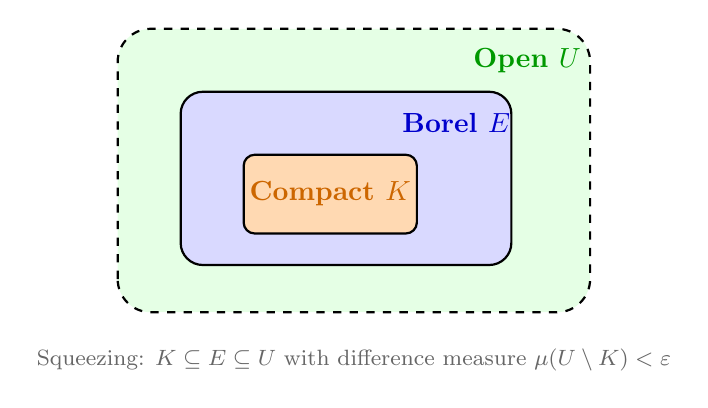
\begin{tikzpicture}[font=\small]
  % Outer open set U
  \draw[thick, dashed, fill=green!10, rounded corners=12pt] (0,0) rectangle (6.0, 3.6);
  \node[green!60!black, font=\bfseries] at (5.2, 3.2) {Open $U$};

  % Target Borel set E
  \draw[thick, fill=blue!15, rounded corners=8pt] (0.8, 0.6) rectangle (5.0, 2.8);
  \node[blue!80!black, font=\bfseries] at (4.3, 2.4) {Borel $E$};

  % Inner compact set K
  \draw[thick, fill=orange!30, rounded corners=4pt] (1.6, 1.0) rectangle (3.8, 2.0);
  \node[orange!80!black, font=\bfseries] at (2.7, 1.5) {Compact $K$};

  \node[font=\footnotesize, text=gray!80!black, align=center] at (3.0, -0.6) 
    {Squeezing: $K \subseteq E \subseteq U$ with difference measure $\mu(U \setminus K) < \varepsilon$};
\end{tikzpicture}
\end{document}